\documentclass[11pt,parskip=full]{scrartcl}%article}
%\setlength{\parskip}{1em}

%%%%%%%%%%%%%%%%%%%%%%
%% PACKAGE INCLUDES %%
%%%%%%%%%%%%%%%%%%%%%%

\usepackage{array}           % For defining \newcolumntype.
\usepackage{amsmath}
\usepackage{amssymb}
\usepackage{amsthm}          % Provides 'proof' environment.
\usepackage[english]{babel}  % For defining 'theorem/corollary/lemma' envs.
\usepackage{bm}              % Provides bold \pi via \bm{}.
\usepackage{booktabs}
\usepackage{hyperref}
\usepackage{todonotes}
\usepackage{enumitem}
\usepackage{mathtools}
\usepackage{caption}         % subtables.
\usepackage{subcaption}      % subtables.
%\usepackage{subfigmat}
\usepackage{comment}
\usepackage{xcolor}          % custom colors.


%%%%%%%%%%%%%%%%%
%% STYLE SETUP %%
%%%%%%%%%%%%%%%%%

% Define some custom colors.
\definecolor{mylinkcolor}{RGB}{000, 114, 166}
\definecolor{mycitecolor}{RGB}{255, 154, 071}
\definecolor{myurlcolor}{RGB}{000, 114, 166}
\definecolor{C0}{RGB}{31,119,180}  % muted blue
\definecolor{C1}{RGB}{255,127,14}  % safety orange
\definecolor{C2}{RGB}{44,160,44}   % cooked asparagus green
\definecolor{C3}{RGB}{214,39,40}   % brick red


% Set itemize format.
\setitemize{noitemsep,topsep=-5pt,parsep=5pt,partopsep=0pt}

% Define column types that allow fixed width params.
\newcolumntype{L}[1]{>{\raggedright\let\newline\\\arraybackslash\hspace{0pt}}m{#1}}
\newcolumntype{C}[1]{>{\centering\let\newline\\\arraybackslash\hspace{0pt}}m{#1}}
\newcolumntype{R}[1]{>{\raggedleft\let\newline\\\arraybackslash\hspace{0pt}}m{#1}}

% Color setup for hyperlinks/references/citations/urls.
\hypersetup{
    colorlinks,
    linkcolor={mylinkcolor},
    citecolor={mycitecolor},
    urlcolor={myurlcolor}
}

% Specify hyphenation of words on line break.
\hyphenation{Figure Table Chapter Section}



%%%%%%%%%%%%
%% MACROS %%
%%%%%%%%%%%%

% Set default font family to sans-serif.
\renewcommand*{\familydefault}{\sfdefault}

\newcommand*{\ie}{i.e., }
\newcommand*{\eg}{e.g., }
\newcommand*{\wrt}{with respect to }

\newcommand*{\Min}{\mathrm{min}}
\newcommand*{\Max}{\mathrm{max}}

\newcommand*{\tokens}{\mathcal{T}}          % Set of tokens.
\newcommand*{\orders}{\mathcal{O}}          % Set of orders.
\newcommand*{\buyorders}{\mathcal{O}^b}     % Set of buy orders.
\newcommand*{\sellorders}{\mathcal{O}^s}    % Set of sell orders.
\newcommand*{\itokens}{\mathcal{I}^t}       % Set of token indices.
\newcommand*{\itokenpairs}{\mathcal{I}^p}   % Set of token index pairs.
\newcommand*{\iutokenpairs}{\tilde{\mathcal{I}}^p}   % Set of token index pairs.
\newcommand*{\iorders}{\mathcal{I}^o}       % Set of order indices.
\newcommand*{\ibuyorders}{\mathcal{I}^b}    % Set of buy order indices.
\newcommand*{\isellorders}{\mathcal{I}^s}   % Set of sell order indices.

% Macros for references etc.
\newcommand*{\figref}[1]{\hyperref[{#1}]{Figure~\ref*{#1}}}
\newcommand*{\tabref}[1]{\hyperref[{#1}]{Table~\ref*{#1}}}
\newcommand*{\secref}[1]{\hyperref[{#1}]{Section~\ref*{#1}}}
\newcommand*{\subsecref}[1]{\hyperref[{#1}]{Section~\ref*{#1}}}
\newcommand*{\thmref}[1]{\hyperref[{#1}]{Theorem~\ref*{#1}}}
\newcommand*{\crlref}[1]{\hyperref[{#1}]{Corollary~\ref*{#1}}}
\newcommand*{\lemref}[1]{\hyperref[{#1}]{Lemma~\ref*{#1}}}

% Macros for theorems|corollaries|lemmas|observations.
\newtheorem{theorem}{Theorem}[section]
\newtheorem{corollary}{Corollary}[theorem]
\newtheorem{lemma}[theorem]{Lemma}
\newtheorem{observation}[theorem]{Observation}

%%%%%%%%%%%%%%
%% DOCUMENT %%
%%%%%%%%%%%%%%

\title{
  Multi-token Batch Auctions with Uniform Clearing Prices\\
  - \\
  \Large Features and Models}
\author{Tom Walther \\ tom@gnosis.pm}

\date{\today}



\begin{document}

\maketitle


\begin{abstract}
  This document describes the problem of multi-token batch auctions with uniform clearing prices
  as a price-finding mechanism proposed for a decentralized token trading platform.
  Moreover, it contains solution approaches based on combinatorial optimization formulations,
  as well as some computational results.
%\footnote{... footnote ...}.
\end{abstract}

%\todo[inline,caption={}]{
%  \begin{itemize}
%    \item computational results for MIP\{2|3\}
%  \end{itemize}
%}


\tableofcontents

\newpage
\section{Introduction}
\label{sec:introduction}

In continuous-time token exchange mechanisms, orders are typically collected in order books of two
tokens that are traded against each other.
A trade happens whenever a buy order of one token is matched by a sell order of the other, \ie if
there exists an exchange rate that satisfies the limit prices stated in the respective orders.
In a setting of multiple tradeable tokens, one separate order book is required for every token pair
combination.
This may significantly limit liquidity for less frequently traded token pairs and lead to large
bid-ask spreads and low trading volumes.

In our approach, we want to collect orders for a set of multiple tokens in a single joint order
book and compute exchange prices for all token pairs simultaneously at the end of discrete time
intervals (\emph{multi-token batch auction}).
Trades between the same token pairs are then all executed at the same exchange rate (\emph{uniform
clearing price}).
Moreover, this mechanism enables so-called \emph{ring trades}, where orders are matched along
cycles of tokens.
In order to exclude arbitrage opportunities, we require prices to be consistent along such cycles,
\ie we want the constraint
\begin{align}
  p_{j|k} \cdot p_{k|l} = p_{j|l}
  \label{eq:arbitrage_freeness}
\end{align}
to be satisfied for the exchange rates $p_{j|k}, p_{j|l}, p_{k|l}$ between all tokens
$ \tau_j, \tau_k, \tau_l $.

The concept of frequent batch auctions aiming at reducing arbitrage and improving liquidity has
been investigated extensively in \cite{BUDISH-ET-AL_2015:HFT}.
Moreover, the advantages of uniform-price clearing have been discussed in 
\cite{ENGELBRECHT-KAHN_1998:multi-unit-auctions}.
In this document, we want to describe the problem of determining uniform clearing prices for all
pairs of tokens involved in a multi-token batch auction process, and present a mixed-integer
programming (MIP) solution approach.


\clearpage
\section{Problem statement}
\label{sec:problem}

In this section, we want to give a high-level description of the problem that we are investigating,
thereby introducing some general notation and giving an overview of the constraints and properties
that we will focus on.

\subsection{Model components}
\label{subsec:model_components}

\paragraph{Tokens \& exchange rates}

Let $ \tokens := \{ \tau_1 \ldots \tau_n \} $ denote the set of the $ n $ tokens that we want to
consider.
Additionally, we introduce an artificial token~$ \tau_0 $ that shall be referred to as 
\emph{reference token}, which will become important in our modelling approaches later on in 
\secref{sec:models}.
For convenience of notation, we use $ \mathcal{I}^t := \{ 1 \ldots n \} $ to denote the indices
of our token set.

The pairwise exchange rates between two tokens $ \tau_j $ and $ \tau_k $ will be denoted by
$ p_{j|k} $, meaning the price of one unit of $ \tau_j $ measured in units of $ \tau_k $.
As an example, if $ p_{j|k} = 10 $, one would need to pay an amount of $ 10 $ units of $ \tau_k $
in order to purchase one unit of $ \tau_j $.

\paragraph{Orders}

Let there be a set $ \orders = \{ \omega_1 \ldots \omega_N \} $ of $ N $ orders in the batch to be
processed and let $ \iorders := \{ 1 \ldots N \} $ denote its set of indices.
Every order is specified as a tuple $ \omega = (j,k,\overline{x},\overline{y},\pi) $ whose elements
are to be understood as follows:
\begin{align*}
  j &\in \itokens &&
    \ldots \quad \tau_j \> \text{is the token to be bought,}\\
  k &\in \itokens &&
    \ldots \quad \tau_k \> \text{is the token to be sold,}\\
  \overline{x} &\in \mathbb{R}_{\ge 0} \cup \{+\infty\} &&
    \ldots \quad \text{maximum amount of} \> \tau_j \> \text{to be bought,}\\
  \overline{y} &\in \mathbb{R}_{\ge 0} \cup \{+\infty\} &&
    \ldots \quad \text{maximum amount of} \> \tau_k \> \text{to be sold,}\\
  \pi &\in \mathbb{R}_{>0} \cup \{+\infty\} &&
    \ldots \quad \text{limit exchange rate for order execution, \ie} \> p_{j|k} \le \pi.
\end{align*}

Using this universal notation, we can express a variety of different order types:
\begin{enumerate}
  \item \emph{Limit buy orders} as $(j,k,\overline{x},+\infty,\pi)$
    with $\overline{x} < +\infty$ and $\pi < +\infty$:
  \vspace{.2cm}\newline
  "Buy (at most) $\overline{x}$ units of token~$\tau_j$ for $\tau_k$
  if the exchange rate~$p_{j|k}$ is at most $\pi$".
  \vspace{.2cm}\newline
  The market participant sets a fixed maximum buy amount~$\overline{x}$
  and a limit exchange rate~$\pi$, whereas the amount of tokens~$\tau_k$ to be spent is
  implicitely bounded by $\overline{x} \cdot \pi$.

  \item \emph{Limit sell orders} as $(j,k,+\infty,\overline{y},\pi)$
    with $\overline{y} < +\infty$ and $\pi < +\infty$:
  \vspace{.2cm}\newline
  "Sell (at most) $\overline{y}$ units of token~$\tau_k$ for $\tau_j$
  if the exchange rate~$p_{k|j}$ is at least $1/\pi$".
  \vspace{.2cm}\newline
  The market participant sets a fixed maximum sell amount~$\overline{y}$
  and a limit exchange rate~$\pi$, but does not have a limit on the amount of tokens~$\tau_j$
  to be obtained.
  The higher the exchange rate~$p_{k|j}$, the more tokens~$\tau_j$ the trader receives.

  \item \emph{Double-sided limit orders} as $(j,k,\overline{x},\overline{y},\pi)$
    with $\overline{x} < +\infty$, $\overline{y} < +\infty$ and $\pi < +\infty$:
  \vspace{.2cm}\newline
  "Spend (at most) $\overline{y}$ units of token~$\tau_k$
  to buy (at most) $\overline{x}$ units of token~$\tau_j$
  if the exchange rate~$p_{j|k}$ is at most $\pi$".
  \vspace{.2cm}\newline
  The market participant sets both a fixed maximum buy amount~$\overline{x}$
  and sell amount~$\overline{y}$ as well as a limit price $\pi$.
  In contrast to a standard limit sell order, the trader prefers spending less tokens~$\tau_k$
  over receiving more tokens~$\tau_j$ in case the exchange rate~$p_{j|k}$ is significantly
  more favorable as anticipated.

  \item \emph{Market buy orders} as $(j,k,\overline{x},+\infty,+\infty)$
    with $\overline{x} < +\infty$:
  \vspace{.2cm}\newline
  "Buy (at most) $\overline{x}$ units of token~$\tau_j$ for $\tau_k$ at market rate.
  \vspace{.2cm}\newline
  The market participant only sets a fixed maximum buy amount~$\overline{x}$
  and is ready to buy tokens~$\tau_j$ at any market rate.

  \item \emph{Market sell orders} as $(j,k,+\infty,\overline{y},+\infty)$
    with $\overline{y} < +\infty$:
  \vspace{.2cm}\newline
  "Sell (at most) $\overline{y}$ units of token~$\tau_k$ for $\tau_j$ at market rate.
  \vspace{.2cm}\newline
  The market participant only sets a fixed maximum sell amount~$\overline{y}$
  and is ready to sell tokens~$\tau_k$ at any market rate.

  \item \emph{Double-sided market orders} as $(j,k,\overline{x},\overline{y},+\infty)$
    with $\overline{x} < +\infty$ and $\overline{y} < +\infty$:
  \vspace{.2cm}\newline
  "Spend (at most) $\overline{y}$ units of token~$\tau_k$
  to buy (at most) $\overline{x}$ units of token~$\tau_j$
  regardless of the exchange rate~$p_{j|k}$ .
  \vspace{.2cm}\newline
  The market participant sets both a fixed maximum buy amount~$\overline{x}$
  and sell amount~$\overline{y}$, but no limit price $\pi$.
  Hence, the trader expresses a willingness to a buy up to a certain amount of $\tau_j$ independent
  of the price per unit, but limits the total amount of $\tau_k$ that needs to be paid.
\end{enumerate}

\figref{fig:buy_sell_demand} illustrates the characteristic buy- and sell-profiles of the
three different limit order types depending on the exchange rate~$p_{j|k}$.

Please note that orders with $j=k$, \ie identical buy- and sell-token, imply trading with oneself.
While such orders similarly fit into all of the following theory and models as any other orders,
it might make sense to explicitely require $j \neq k$ from a semantic perspective.

\begin{figure}
  \begin{subfigure}{0.45\textwidth}
    \begin{tikzpicture}

  % Horizontal axis for p_{j|k}.
  \draw[->] (0,0) -- (4.2,0) node[anchor=west] {$p_{j|k}$};
  \draw (3.5,0) node[anchor=north] {$\pi$};

  \draw[->] (0,3) -- (4.2,3) node[anchor=west] {$p_{j|k}$};
  \draw (3.5,0) node[anchor=north] {$\pi$};

  % Limit price.
  \draw[dotted] (3.5,0) -- (3.5,2.5);
  \draw[dotted] (3.5,3) -- (3.5,5.5);

  % Vertical axes.
  \draw[-] (0,0) -- (0,2.5);
  \draw[very thick,color=C1] (0,1) -- (3.5,2); % sell demand
  \node[mark size=2pt,color=C1] at (3.5,2) {\pgfuseplotmark{*}};
  \draw[very thick,color=C1] (3.5,0.05) -- (4,0.05); % sell demand
  \draw (0,1) node[anchor=east] {$\overline{x} \cdot p_{j|k}$};

  \draw[-] (0,3) -- (0,5.5);
  \draw[very thick,color=C0] (0,4.5) -- (3.5,4.5); % buy demand
  \node[mark size=2pt,color=C0] at (3.5,4.5) {\pgfuseplotmark{*}};
  \draw[very thick,color=C0] (3.5,3.05) -- (4,3.05); % buy demand
  \draw (0,4.5) node[anchor=east] {$\overline{x}$};

\end{tikzpicture}
    \caption{Limit buy order}
  \end{subfigure}
  \hfill
  \begin{subfigure}{0.45\textwidth}
    \begin{tikzpicture}

  % Horizontal axis for p_{j|k}.
  \draw[->] (0,0) -- (4.2,0) node[anchor=west] {$p_{j|k}$};
  \draw (3.5,0) node[anchor=north] {$\pi$};

  \draw[->] (0,3) -- (4.2,3) node[anchor=west] {$p_{j|k}$};
  \draw (3.5,0) node[anchor=north] {$\pi$};

  % Limit price.
  \draw[dotted] (3.5,0) -- (3.5,2.5);
  \draw[dotted] (3.5,3) -- (3.5,5.5);

  % Vertical axes.
  \draw[-] (0,0) -- (0,2.5);
  \draw[very thick,color=C1] (0,1.5) -- (3.5,1.5); % sell demand
  \node[mark size=2pt,color=C1] at (3.5,1.5) {\pgfuseplotmark{*}};
  \draw[very thick,color=C1] (3.5,0.05) -- (4,0.05); % sell demand
  \draw (0,1.5) node[anchor=east] {$\overline{y}$};

  \draw[-] (0,3) -- (0,5.5);
  \draw[very thick,color=C0] (0,5) parabola[bend at end] (3.5,3.75); % buy demand
  \node[mark size=2pt,color=C0] at (3.5,3.75) {\pgfuseplotmark{*}};
  \draw[very thick,color=C0] (3.5,3.05) -- (4,3.05); % buy demand
  \draw (0,5) node[anchor=east] {$\frac{\overline{y}}{p_{j|k}}$};

\end{tikzpicture}
    \caption{Limit sell order}
  \end{subfigure}

  \vspace{.8cm}
  \begin{subfigure}{0.45\textwidth}
    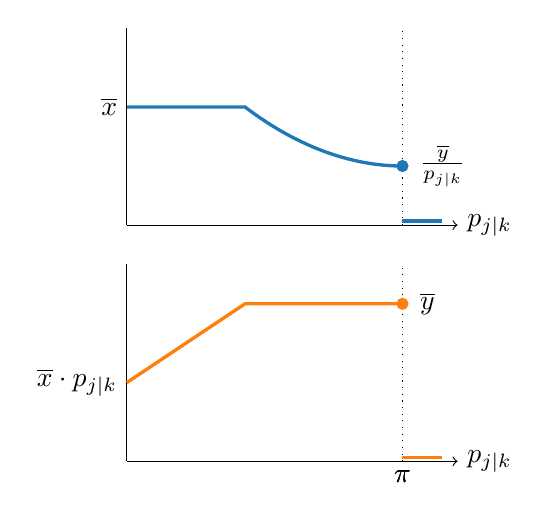
\begin{tikzpicture}

  % Horizontal axis for p_{j|k}.
  \draw[->] (0,0) -- (4.2,0) node[anchor=west] {$p_{j|k}$};
  \draw (3.5,0) node[anchor=north] {$\pi$};

  \draw[->] (0,3) -- (4.2,3) node[anchor=west] {$p_{j|k}$};
  \draw (3.5,0) node[anchor=north] {$\pi$};

  % Limit price.
  \draw[dotted] (3.5,0) -- (3.5,2.5);
  \draw[dotted] (3.5,3) -- (3.5,5.5);

  % Vertical axes.
  \draw[-] (0,0) -- (0,2.5);
  \draw[very thick,color=C1] (0,1) -- (1.5,2) -- (3.5,2); % sell demand
  \node[mark size=2pt,color=C1] at (3.5,2) {\pgfuseplotmark{*}};
  \draw[very thick,color=C1] (3.5,0.05) -- (4,0.05); % sell demand
  \draw (0,1) node[anchor=east] {$\overline{x} \cdot p_{j|k}$};
  \draw (3.6,2) node[anchor=west] {$\overline{y}$};

  \draw[-] (0,3) -- (0,5.5);
  \draw[very thick,color=C0] (0,4.5) -- (1.5,4.5) parabola[bend at end] (3.5,3.75); % buy demand
  \node[mark size=2pt,color=C0] at (3.5,3.75) {\pgfuseplotmark{*}};
  \draw[very thick,color=C0] (3.5,3.05) -- (4,3.05); % buy demand
  \draw (0,4.5) node[anchor=east] {$\overline{x}$};
  \draw (3.6,3.75) node[anchor=west] {$\frac{\overline{y}}{p_{j|k}}$};

\end{tikzpicture}
    \caption{Double-sided limit order}
  \end{subfigure}
  \hfill
  \begin{subfigure}{0.45\textwidth}
    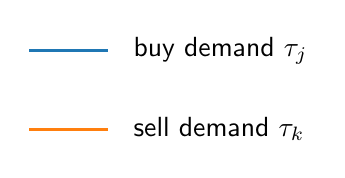
\begin{tikzpicture}
      \draw[very thick,color=C0] (1,1) -- (2,1); % buy demand
      \draw (2.2,1) node[anchor=west] {buy demand $\tau_j$};
      \draw[very thick,color=C1] (1,0) -- (2,0); % buy demand
      \draw (2.2,0) node[anchor=west] {sell demand $\tau_k$};
    \end{tikzpicture}
  \end{subfigure}
  \caption{
    Buy- and sell-profiles for limit orders (types 1/2/3).
    The graphs show the transacted amounts of tokens with respect to the exchange rate~$p_{j|k}$
    in the case that the order is fully executed.
    The maximum buy-amount is computed as $\min\{\overline{x},\overline{y}/p_{j|k}\}$, whereas the
    maximum sell-amount equals $\min\{\overline{y},\overline{x} \cdot p_{j|k}\}$.
    The graphs look similar for market orders (types 4/5/6), with the only difference being the
    absence of a limit price~$\pi$.}
  \label{fig:buy_sell_demand}
\end{figure}

\vspace{.3cm}
\begin{observation}
  Assuming that the trader has constant utility for an arbitrary amount of buy-tokens~$\tau_j$,
  the following argument can be used to convert a limit buy order to a limit sell order:
  Consider a limit buy order $ (j,k,\overline{x},+\infty,\pi) $, which reveals that the trader
  would be ready to sell at most $ \pi \cdot \overline{x} $ tokens $ \tau_k $ in exchange for
  tokens $ \tau_j $.
  Then, the trader would not object to receiving more than $ \overline{x} $ tokens $ \tau_j $ for a
  maximum of $ \pi \cdot \overline{x} $ tokens $ \tau_k $, \ie if the exchange rate $ p_{j|k} $ is
  lower than $ \pi $.
  Hence, the trader would only benefit from submitting a sell order
  $ (k,j,+\infty,\pi \cdot \overline{x},\frac{1}{\pi}) $.
\end{observation}


\subsection{Variables}
\label{subsec:variables}

The goal of our approach is to determine the exchange rates between all token pairs that allow for the best possible matching of orders (according to one of the metrics suggested in \secref{subsec:objectives}).
Hence, both the exchange rates as well as the traded token amounts per order represent the generic set of variables for our problem.

For every order $\omega = (j,k,\overline{x},\overline{y},\pi) \in \orders$, we introduce two variables $x \in \mathbb{R}_{\ge 0}$ and $y \in \mathbb{R}_{\ge 0}$ that denote the amount of tokens~$\tau_j$ bought and the amount of tokens~$\tau_k$ sold, respectively.
Obviously, these need to satisfy the specified order amounts, \ie $x \le \overline{x}$ and $y \le \overline{y}$.

Working directly with the exchange rates~$p_{j|k}$ as variables for all token pairs $(\tau_j,\tau_k)$ leads to nonlinear dependencies in the constraints that we are aiming to satisfy.
Hence, for every token~$\tau_j \in \tokens$, we introduce a new variable $p_j := p_{j|0}$ denoting the price of~$\tau_j$ expressed in units of the reference token~$\tau_0$.
The price~$p_0$ of the reference token itself can be fixed to some constant in order to remove the excess degree of freedom.
Without loss of generality, we will use~$p_0 = 1$ throughout this paper.
The relationship between the exchange rate and the price variables will be derived in \secref{subsec:constraints}.


\subsection{Constraints}
\label{subsec:constraints}

The solution that we are trying to find needs to satisfy several requirements that can be stated on a high level as follows:
\begin{itemize}
  \item \emph{(maximum buy and sell amount)}:\\
  for every order $\omega = (j,k,\overline{x},\overline{y},\pi) \in \orders$:
  the amount of tokens bought and sold must not exceed the specified limits, \ie $x \le \overline{x}$ and $y \le \overline{y}$.
  \item \emph{(limit price)}:\\
  for every order $\omega = (j,k,\overline{x},\overline{y},\pi) \in \orders$:
  the order can only be executed (fully or fractionally) if the exchange rate satisfies the limit price, \ie $ p_{j|k} \le \pi $.
  \item \emph{(uniform clearing price)}:\\
  for every order $\omega = (j,k,\overline{x},\overline{y},\pi) \in \orders$:
  the order is executed using the exchange rate~$p_{j|k}$ which is uniquely determined for each token pair~$(\tau_j,\tau_k)$, \ie, $y = x \cdot p_{j|k}$.
  \item \emph{(token balance)}:\\
  for every token $ \tau \in \tokens $: 
  the amount of tokens $ \tau $ that were bought must equal the amount of tokens $ \tau $ that were sold across all orders.
  \item \emph{(price coherence)}:\\
  for all token pairs $ (\tau_j,\tau_k) $: $ p_{j|k} \cdot p_{k|j} = 1 $.
  \item \emph{(arbitrage freeness)}:\\
  for all token triples $ (\tau_j,\tau_k,\tau_l) $: $ p_{j|k} \cdot p_{k|l} = p_{j|l} $.
\end{itemize}

\vspace{.8cm}
\begin{lemma}
  (arbitrage freeness) $ \Rightarrow $ (price coherence).
\end{lemma}
\vspace{-.8cm}
\begin{proof}
  Consider three tokens $ \{\tau_j,\tau_k,\tau_l\} \subset \tokens $.
  We apply the arbitrage-freeness condition twice:
  \begin{align*}
    \text{(i)}  \>\> p_{j|k} \cdot p_{k|l} &= p_{j|l} \\
    \text{(ii)} \>\> p_{j|l} \cdot p_{l|k} &= p_{j|k}
  \end{align*}
  Inserting (i) into (ii) and assuming prices to be strictly positive yields
  \begin{align*}
    p_{j|k} \cdot p_{k|l} \cdot p_{l|k} = p_{j|k}
    \qquad \Leftrightarrow \qquad
    p_{k|l} \cdot p_{l|k} = 1
  \end{align*}
\end{proof}
\vspace{-.4cm}

Notice that the above constraints also imply $ p_{j|j} = 1 $ for every token~$ \tau_j \in \tokens $.

\paragraph{(Relative) Exchange rates vs. (absolute) token prices}

Moreover, the arbitrage-freeness and price-coherence conditions help establish a relation between the exchange rate variable~$p_{j|k}$ for token pair~$(\tau_j,\tau_k)$ and the price variables~$p_j$ and $p_k$ for the individual tokens (as defined in \secref{subsec:variables}):
\begin{align}
  p_{j|k} = p_{j|0} \cdot p_{0|k} = \frac{p_{j|0}}{p_{k|0}} = \frac{p_j}{p_k}.
  \label{eq:price_decomposition}
\end{align}
Consequently, working with token price variables rather than pairwise exchange rates automatically guarantees arbitrage-freeness across all tokens.
Moreover, the uniform clearing price condition can be rewritten as $\frac{p_j}{p_k} \le \pi$, while the uniform clearing price constraint becomes $x \cdot p_j = y \cdot p_k$.
Both conditions together yield an equivalent expression for the limit price: $x \cdot \pi \ge y$.

\paragraph{Reference token}

We now have some freedom to decide what precisely the artificial reference token should represent.
For example, we could select one particular $ \tau_j \in \tokens $ to be the \emph{numeraire}, \ie
\begin{subequations}
\begin{align}
  p_0 &= p_j.
  \label{eq:refToken_1}
\end{align}
Then, all trading volume would be computed \wrt $ \tau_j $, making this the principal token in the batch auction.
Alternatively and more generally, we could also identify $ \tau_0 $ with a weighted sum of all
participating tokens in $ \tokens $, \ie
\begin{align}
  p_0 &= \sum\limits_{j \in \itokens} \gamma_j \cdot p_j,
  \label{eq:refToken_2}
\end{align}
\end{subequations}
with weights $ \gamma_j > 0 $.
This way, it would be possible to give similar importance to all tokens, \eg by using weights
$ \gamma_j = 1 / (n \cdot p_j^\mathrm{old}) $, where $ p_j^\mathrm{old} $ denotes the price of
token $ \tau_j $ found in the previous batch auction iteration.

\vspace{.2cm}
\begin{observation}
The choice of representation of the reference token has an influence on the solution.
This can be seen by considering a single token pair $ (\tau_j,\tau_k) $ with only two buy orders
$ \omega_1 = (j,k,1.0,+\infty,2.0) $ and $ \omega_2 = (k,j,1.5,+\infty,1.0) $.
Both orders can be matched if $ p_{j|k} \in [1,2] $.
However, if we choose token $ \tau_j $ to be the reference token, a maximum of $ 1.0 \, \tau_j $
can be transacted for prices $ p_{j|k} \in [1,1.5] $, whereas the maximum trading volume of
$ 1.5 \, \tau_k $ can be achieved when $ p_{j|k} \in [1.5,2] $.
\end{observation}


\subsection{Objectives}
\label{subsec:objectives}

As mentioned previously, for a given batch of orders~$\mathcal{O}$ on the set of tokens~$\mathcal{T}$, it is our goal to determine the exchange rates~$p_{j|k}$ for all token pairs~$(\tau_j,\tau_k)$ together with an order matching such that a certain optimization criterion is maximized.
We are considering the following three objective functions:

\paragraph{Trading volume}

The most obvious optimization criterion would be to target a solution that enables as much trade as possible.
Due to their different prices, we can not simply maximize for the total number of tokens traded, but need a common scale as a measure of value.
Hence, for every order~$\omega = (j,k,\overline{x},\overline{y},\pi) \in \orders$, a new variable~$v \in \mathbb{R}_{\ge 0}$ representing the \emph{trading volume} is introduced, defined as
\begin{align}
  v := x \cdot p_j = y \cdot p_k.
  \label{eq:volume}
\end{align}
In words, the trading volume measures the value of all transactions in terms of units of the reference token~$\tau_0$.
The objective function comprises the sum of the trading volumes of all orders.

\paragraph{Social surplus/welfare}

As a downside, the trading volume does not take the limit prices of orders into account.
For orders on the same token pair, traders might expect the ones with the best limit prices to be filled with preference over those whose limit prices are very close to the determined exchange rate.
A measure that captures the valuation of the order executed by the trader is called \emph{social surplus} or \emph{social welfare}, denoted by a variable~$w \in \mathbb{R}_{\ge 0}$ per order.
It uses the amount~$x$ of tokens~$\tau_j$ bought, determines how many tokens~$\tau_k$ the trader would have been ready to spend (via the limit price~$\pi$), and values this amount with the token price~$p_k$:
\begin{align}
  w &:= x \cdot \pi \cdot p_k.
  \label{eq:welfare}
\end{align}
Again, the objective function is the sum of all $w$.

\paragraph{Trader's utility}

Finally, combining trading volume and valuation, another measure called \emph{trader's utility} could be used as objective.
We will denote it by $u \in \mathbb{R}_{\ge 0}$ and it can be considered in two variants:
\begin{itemize}
  \item the difference between the amount that the trader would have been ready to spend for an amount of~$x$ buy-tokens~$\tau_j$ and the amount~$y$ that is actually spent (weighted by the price~$p_k$ of the sell-token~$\tau_k$):
  \begin{subequations}
  \begin{align}
    u := (x \cdot \pi - y) \cdot p_k
    \label{eq:utility_a}
  \end{align}
  \item the difference between the amount~$x$ of tokens~$\tau_j$ bought and the amount that the trader would have accepted as a minimum for spending~$y$ tokens~$\tau_k$ (now weighted by the price~$p_j$):
  \begin{align}
    u := (x - y/\pi) \cdot p_j
    \label{eq:utility_b}
  \end{align}
  \label{eq:utility}
  \end{subequations}
\end{itemize}

Notice that definition \eqref{eq:utility_a} yields $u = w - v$.


\begin{comment}
\paragraph{Properties}

Here is a list of research questions that we would like to answer.

\begin{itemize}
  \item In an optimal solution, is it guaranteed that orders can always be fully executed if their
  limit prices are strictly higher (buy order) or lower (sell order) than the exchange rate between
  the respective token pair?
  If true, we would only need to resort to partially executing orders if the execution price is
  equal to the limit price.
  \item What is the impact of optimizing the trading volume vs. the traders' welfare?
\end{itemize}
\end{comment}

\newpage
\subsection{Example}

A typical instance of our batch auction problem could look like shown in 
\figref{fig:order-token-graph}.
It is assumed that some token pairs will encounter high trading demand whereas other will only
rarely be traded on.

\begin{figure}[h!]
  \centering
  \includegraphics[width=.75\textwidth]{figures/token_order_graph.png}
  \caption{Token-order-graph representing a multi-token batch auction instance. Nodes correspond
  to tokens (with their size indicating the trading demand), the thickness of an edge represents 
  the number of orders placed on the respective token pair.}
  \label{fig:order-token-graph}
\end{figure}


\clearpage
\section{Models and Formulations}
\label{sec:models}

In this section, we want to present and discuss several solution approaches for our batch auction
problem in terms of mathematical optimization formulations.

\vspace{-.2cm}
\paragraph{Data}

At first, we will express all information given in the orders in terms of data matrices and
vectors, aiming at being able to write down a complete optimization model.
Recall that every order $ \omega \in \orders $ is defined by a tuple
$ (j,k,\overline{x},\overline{y},\pi) $ specifying the buy- and sell-token, the maximum amount of
tokens to be bought and sold, as well as the limit price.

We introduce two data matrices
\begin{align*}
  \mathbf{T}^b &\in \{0,1\}^{N \times n} && \text{with} & \mathbf{T}^b \ni t^b_{i,j} = 1
  &\Leftrightarrow
  \text{token} \; \tau_j \; \text{to be bought in order} \; \omega_i \\
  \mathbf{T}^s &\in \{0,1\}^{N \times n} && \text{with} & \mathbf{T}^s \ni t^s_{i,j} = 1
  &\Leftrightarrow
  \text{token} \; \tau_j \; \text{to be sold in order} \; \omega_i
\end{align*}
For now, we are only considering orders of one token against one other, so there must be exactly
one entry equal to $ 1 $ per row (order) in both $ \mathbf{T}^b $ and $ \mathbf{T}^s $.
An extension to so-called \emph{basket orders} where multiple tokens are traded against multiple
others is discussed as an extension \secref{subsec:basket_orders}.

Let $ (\overline{x}_i) =: \overline{\mathbf{x}} \in \mathbb{R}^N_{\ge 0} $ and 
$ (\overline{y}_i) =: \overline{\mathbf{y}} \in \mathbb{R}^N_{\ge 0} $ contain the maximum amounts
of tokens to be bought and sold, respectively, in every order.

Finally, the limit prices of all orders shall be stored as vector
$ (\pi_i) =: \bm{\pi} \in \mathbb{R}^N_{\ge 0} $, where $ \pi_i \in \bm{\pi} $ refers to the
exchange rate between the respective buy- and sell-tokens at which order $ \omega_i $ may be
executed (according to the definition in \subsecref{sec:problem}).

\vspace{-.2cm}
\paragraph{Variables}

Let $(p_j) =: \mathbf{p} \in \mathbb{R}^n_{> 0}$ be a vector containing all token prices to be determined.
For the orders, we use the following notation:
\begin{align*}
  (x_i) &=: \mathbf{x} \in \mathbb{R}^N_{\ge 0} && \ldots\>\text{number of tokens bought}\\
  (y_i) &=: \mathbf{y} \in \mathbb{R}^N_{\ge 0} && \ldots\>\text{number of tokens sold}\\[2mm]
  (v_i) &=: \mathbf{v} \in \mathbb{R}^N_{\ge 0} && \ldots\>\text{trading volume}\\
  (w_i) &=: \mathbf{w} \in \mathbb{R}^N_{\ge 0} && \ldots\>\text{social surplus}\\
  (u_i) &=: \mathbf{u} \in \mathbb{R}^N_{\ge 0} && \ldots\>\text{trader's utility}\\
\end{align*}


\paragraph{Constraints}

We need to distinguish two different behaviours for every order: Either the exchange rate
on the respective token pair satisfies its limit price (and thus the order may be executed), or it
does not (thus the order needs to remain untouched).
Optionally, we could incorporate a minimum fraction of execution, denoted by a parameter
$r^\Min \in [0,1]$, for the case that an order may be executed.
This parameter may be set globally for all orders, or for every order individually.
In the following, however, we assume that there is no minimum order execution fraction imposed,
\ie $r^\Min = 0$.
We will discuss the impact of $r^\Min>0$ in \secref{sec:extensions}.

In general, for an order given as $ \omega = (j,k,\overline{x},\overline{y},\pi) $, this yields
the following two sets of constraints:
\begin{align}
  \mathfrak{C}^1 := \left\{
  \begin{array}{rll}
    x &\le & \overline{x} \\
    y &\le & \overline{y} \\
    x \cdot p_j &= & y \cdot p_k \\[1mm]
    \frac{p_j}{p_k} &\le & \pi
  \end{array}
  \right\}
  \quad
  \text{and}
  \quad
  \mathfrak{C}^0 := \left\{
  \begin{array}{rll}
    x &= & 0 \\
    y &= & 0 \\[1mm]
    \frac{p_j}{p_k} &> & \pi
  \end{array}
  \right\}
  \label{eq:order_model_generic}
\end{align}

\paragraph{Objective}

As introduced in \secref{subsec:objectives}, we consider three different objectives:
\begin{align*}
  && &\max\sum_{i \in \iorders} v_i && \ldots\>\text{total trading volume}&&\\
  && &\max\sum_{i \in \iorders} w_i && \ldots\>\text{total social surplus}&&\\
  && &\max\sum_{i \in \iorders} u_i && \ldots\>\text{total traders' utility}&&
\end{align*}


\paragraph{Optional conditions}

In some situations, it might make sense to bound the deviation of the new exchange rates $p_{j|k}$ from the previously computed exchange rates $ p_{j|k}^\mathrm{old} $.
Therefore, let $ p^\mathrm{old}_j $ denote the price of token~$ \tau_j $ found in the previous
batch auction iteration.
Using a maximum fluctuation parameter $ \delta > 0 $, we impose the conditions
\begin{align}
  p_{j|k} \in
  \left[
    \left(\frac{1}{1+\delta}\right) p^\mathrm{old}_{j|k},
    (1+\delta) \, p^\mathrm{old}_{j|k}
  \right]
  \quad &\Leftrightarrow \quad
  \frac{p_j}{p_k} \in
  \left[
    \left(\frac{1}{1+\delta}\right) \frac{p^\mathrm{old}_j}{p^\mathrm{old}_k},
    (1+\delta) \, \frac{p^\mathrm{old}_j}{p^\mathrm{old}_k}
  \right]\notag\\[2mm]
  \quad &\Leftrightarrow \quad
  \begin{cases}
    p_j \ge \left(\frac{1}{1+\delta}\right) \frac{p^\mathrm{old}_j}{p^\mathrm{old}_k} \, p_k
    \\[2mm]
    p_j \le \left(1+\delta\right) \frac{p^\mathrm{old}_j}{p^\mathrm{old}_k} \, p_k
  \end{cases}.
  \label{eq:bounds_xrates}
\end{align}

As an example, $ \delta = 1 $ would set the bounds to half/twice the previous exchange rates.
Note that, if no previous price exists for some token $ \tau_j $, the exchange rate bounds for
token pairs involving $ \tau_j $ could be determined on the basis of the limit prices given in
the respective orders, or simply be set to $ [0,\infty] $.
In theory, the model permits a different fluctuation parameter on every token pair, which allows to
capture real-world expections, \eg, related to the liquidity that is available on each token pair. 

Moreover, it is helpful to incorporate some explicit lower and upper bound for the price of every
token~$ \tau_j $, so let us require $ p_j \in [\underline{p}_j,\overline{p}_j] $.

\begin{lemma}
  For the choice of weights $ \gamma_j = 1 / (n \cdot p_j^\mathrm{old}) $ in \eqref{eq:refToken_2}
  and a given maximum fluctuation parameter $ \delta $, we can impose bounds
  \begin{align}
    p_j \in \left[ \left(\frac{1}{1+\delta}\right) \, p^\mathrm{old}_j, (1+\delta) \,
  p^
  \mathrm{old}_j \right] \forall \, j \in \itokens.
  \end{align}
\end{lemma}
\vspace{-.5cm}
\begin{proof}
  We will prove that the upper bound holds.
  Proving the lower bound works analogous.
  Assume $ p_j > (1+\delta) \, p_j^\mathrm{old} $.
  Then, \eqref{eq:bounds_xrates} yields
  \begin{align*}
    (1+\delta) \, \frac{p^\mathrm{old}_j}{p^\mathrm{old}_k} \, p_k > (1+\delta) \, p_j^\mathrm{old}
    \qquad \Leftrightarrow \qquad p_k > p_k^\mathrm{old}
    \qquad \forall k \neq j.
  \end{align*}
  Inserting into \eqref{eq:refToken_2} leads to a contradiction:
  \begin{align*}
    p_0 = 1
    &= \frac{1}{n \cdot p_j^\mathrm{old}} \, p_j + \sum\limits_{j \neq k \in \itokens}
      \frac{1}{n \cdot p_k^\mathrm{old}} \cdot p_k
    \, > \, \frac{1+\delta}{n} + \sum\limits_{j \neq k \in \itokens} \frac{1}{n} > 1.
  \end{align*}
\end{proof}
\vspace{-.4cm}

All price bounds shall be stored in vectors $\underline{\mathbf{p}}$ and $\overline{\mathbf{p}}$,
respectively.

\newpage
\subsection{Nonlinear programming model}
\label{subsec:NLPmodel}

When looking at the sets of constraints \eqref{eq:order_model_generic}, the most intuitive model seems to be a nonlinear program.
As we will see, it is possible to avoid binary variables.
For simplicity, we will state this (and all the following formulations) using total trading volume as objective function.
The other objectives can be used by inserting and calculating the respective variables.

\begin{subequations}
\begin{align}
  \text{maximize} \quad & \sum\limits_{i \in \iorders} v_i
  \label{eq:nlp_objective}
  \\[2mm]
  \text{subject to} \quad
  \sum\limits_{i \in \iorders} t^b_{i,j} \, x_i
  &= \sum\limits_{i \in \iorders} t^s_{i,j} \, y_i
  && \forall \> j \in \itokens
  \label{eq:nlp_tokenbalance}
  \\[2mm]
  v_i
  &= x_i \sum\limits_{j \in \itokens} t^b_{i,j} \, p_j
  && \forall \> i \in \iorders
  \label{eq:nlp_buyvolume}
  \\[1mm]
  v_i
  &= y_i \sum\limits_{j \in \itokens} t^s_{i,j} \, p_j
  && \forall \> i \in \iorders
  \label{eq:nlp_sellvolume}
  \\[2mm]
  x_i &\le \overline{x}_i
  && \forall \> i \in \iorders
  \label{eq:nlp_limit_x}
  \\[1mm]
  y_i &\le \overline{y}_i
  && \forall \> i \in \iorders
  \label{eq:nlp_limit_y}
  \\[1mm]
  y_i &\le x_i \, \pi_i
  && \forall \> i \in \iorders
  \label{eq:nlp_limit_pi}
  \\[2mm]
  \sum\limits_{j \in \itokens} \gamma_j \cdot p_j
  &= 1
  \label{eq:nlp_reftoken}
  \\[1mm]
  p_j
  &\in [\,\underline{p_j},\overline{p_j}\,]
  && \forall \> j \in \itokens
  \\[1mm]
  x_i, y_i, v_i &\in \mathbb{R}_{\ge 0}
  && \forall \> i \in \iorders
\end{align}
\label{eq:nlp}
\end{subequations}

The objective function \eqref{eq:nlp_objective} maximizes the total volume in terms of units of
the reference token $ \tau_0 $ that is processed with all orders.

Constraint \eqref{eq:nlp_tokenbalance} ensures that the total numbers of tokens bought and sold are
equal for every token across all orders.
The summations in this constraint are only responsible for selecting the correct tokens that are
traded in the orders.

The constraints~\eqref{eq:nlp_buyvolume} and \eqref{eq:nlp_sellvolume} compute the buy and sell
trade volume for every order \wrt the reference token, and make sure these two are equal.
This guarantees that the token prices are chosen such that they are consistent with the traded
amounts of tokens.
If the traded token amounts $ x_i $ and $ y_i $ are zero for some order $ \omega_i $, \ie
$ \omega_i $ is not executed at all, the corresponding trade volume $ v_i $ will be zero as well.
However, this comes at the price of introducing nonlinearity (and even nonconvexity) into the
model.

The maximum token amounts to be bought and sold as specified in every order are incorporated
into the model via the constraints~\eqref{eq:nlp_limit_x} and \eqref{eq:nlp_limit_y}.
Constraint~\eqref{eq:nlp_limit_pi} ensures that the limit price is satisfied, if the order is
to be executed, or that both $ x_i $ and $ y_i $ are set to zero otherwise.
Please note that if either of $\overline{x}$, $\overline{y}$ or $\pi_i$ equals $+\infty$, the
corresponding constraint is trivially satisfied.
Altogether, the constraints~\eqref{eq:nlp_buyvolume}--\eqref{eq:nlp_limit_pi} capture both
cases of \eqref{eq:order_model_generic} simultaneously.

Finally, as described earlier, the constraint \eqref{eq:nlp_reftoken} specifies the representation of the reference token.


\newpage
\subsection{Mixed-integer linear programming model I}
\label{subsec:MIP1}

Since nonlinearity and nonconvexity usually pose strong restrictions on the tractable model size,
we want to proceed with proposing a mixed-integer linear programming (MIP) formulation as an
alternative to the NLP model presented above.
Thereby, the challenge is to find an equivalent linear formulation for 
\eqref{eq:order_model_generic}.

The key idea is to avoid explicitely computing the values $x$ and $y$ for every order~$\omega = (j,k,\overline{x},\overline{y},\pi)$, but only working with the trading volume~$v$ as defined in \eqref{eq:volume} instead.
With uniform clearing prices, $x$ and $y$ can be computed unambiguously from the value of~$v$ later on.
The order constraints \eqref{eq:order_model_generic} can be expressed as follows:
\begin{align}
  \tilde{\mathfrak{C}}^1 := \left\{
  \begin{array}{rlll}
    v &\le & \overline{x} \cdot p_j \\
    v &\le & \overline{y} \cdot p_k \\[1mm]
    \frac{p_j}{p_k} &\le & \pi
  \end{array}
  \right\}
  \quad
  \text{and}
  \quad
  \tilde{\mathfrak{C}}^0 := \left\{
  \begin{array}{rll}
    v &= & 0 \\[1mm]
    \frac{p_j}{p_k} &> & \pi
  \end{array}
  \right\}
  \label{eq:order_model_mip1}
\end{align}

Please notice that this step is not possible for the social surplus~$w$ as in \eqref{eq:welfare} and the trader's utility~$u$ as in \eqref{eq:utility}. 
Hence, we have not found a linear formulation for that maximize these two optimization criteria.

In order to reformulate \eqref{eq:order_model_mip1} in terms of a mixed-integer linear program,
we first introduce a binary variable $ z \in \{0,1\} $ for every order and associate its states to
the constraint sets as $ \{z = 1\} \Leftrightarrow \tilde{\mathfrak{C}}^1 $ and
$ \{z = 0\} \Leftrightarrow \tilde{\mathfrak{C}}^0 $.
For modelling these dependencies, there exist two major strategies that we will apply in the
following:
the \emph{big-M} approach as, \eg mentioned in \cite{BONAMI-ET-AL_2015:indicator-constraints},
as well as \emph{disjunctive programming}, introduced by \textsc{Balas} \cite{BALAS_1979:DP}.

\paragraph{Big-M reformulation}

In the big-M approach, the constraints for both $ \tilde{\mathfrak{C}}^0 $ and
$ \tilde{\mathfrak{C}}^1 $ are modified so that they are equivalent to the original ones if the
binary variable takes the respective value, and are rendered redundant by large-enough constants in
the opposite case.
As for our constraint systems, this translates into:
\begin{subequations}
\begin{align}
  p_j &\le \pi \, p_k + (1-z) (\overline{p}_j - \pi \underline{p}_k) \\
  p_j &\ge (\pi+\varepsilon) \, p_k
    + z \, (\underline{p}_j - (\pi+\varepsilon) \, \overline{p}_k)
    && \text{if } \pi < +\infty \\[1mm]
  v &\le \overline{x} \, p_j \\
  v &\le \overline{x} \, \overline{p}_j \, z
    && \text{if } \overline{x} < +\infty  \\[1mm]
  v &\le \overline{y} \, p_k \\
  v &\le \overline{y} \, \overline{p}_k \, z
    && \text{if } \overline{y} < +\infty
\end{align}
\label{eq:order_model_mip1_bigM}
\end{subequations}

It can easily be verified that substituting $ z=1 $ and $ z=0 $ yields the desired constraints
\eqref{eq:order_model_mip1}.
Notice that the strict inequality $ \frac{p_j}{p_k} > \pi $ in $ \tilde{\mathfrak{C}}^0 $ is
approximated by an inequality $ \frac{p_j}{p_k} \ge \pi + \varepsilon $, with some very small
$ \varepsilon > 0 $.

\paragraph{Disjunctive programming reformulation}

The advantage of the big-M reformulation is its simplicity and compactness.
However, its relaxation is not as tight as it can be, \ie it does not describe the convex hull of
the feasible regions of $ \tilde{\mathfrak{C}}^0 $ and $ \tilde{\mathfrak{C}}^1 $.
This property can be secured in the disjunctive programming approach through the addition of
additional auxiliary variables.

For every order $ \omega = (j,k,\overline{x},\overline{y},\pi) $, we introduce two pairs of
auxiliary nonnegative price variables:
$ p^{b,0}, p^{b,1} $ -- referring to the price $ p_j $ of the buy-token, as well as
$ p^{s,0}, p^{s,1} $ -- referring to the price $ p_k $ of the sell-token.
Then, a disjunctive programming formulation can be given as follows:
\begin{subequations}
\begin{align}
  (1-z) \, \underline{p}_j &\le p^{b,0} \le (1-z) \, \overline{p}_j
    \label{eq:mip1_dp_buyprice_0}\\
  (1-z) \, \underline{p}_k &\le p^{s,0} \le (1-z) \, \overline{p}_k
    \label{eq:mip1_dp_sellprice_0}\\[2mm]
  z \, \underline{p}_j &\le p^{b,1} \le z \, \overline{p}_j
    \label{eq:mip1_dp_buyprice_1}\\
  z \, \underline{p}_k &\le p^{s,1} \le z \, \overline{p}_k
    \label{eq:mip1_dp_sellprice_1}\\[2mm]
  p_j &= p^{b,0} + p^{b,1}
    \label{eq:mip1_dp_buyprice_aggr}\\
  p_k &= p^{s,0} + p^{s,1}
    \label{eq:mip1_dp_sellprice_aggr}\\[2mm]
  p^{b,1} &\le \pi \, p^{s,1}
    \label{eq:mip1_dp_xrate_1}\\
  p^{b,0} &\ge (\pi+\varepsilon) \, p^{s,0}
    \label{eq:mip1_dp_xrate_0}\\[2mm]
  v &\le \overline{x} \, p^{b,1}
    \label{eq:mip1_dp_volume_buy_ub}\\
  v &\le \overline{y} \, p^{s,1}
    \label{eq:mip1_dp_volume_sell_ub}
\end{align}
\label{eq:order_model_mip1_DP}
\end{subequations}

The general idea is that both $p^{b,1}$ and $p^{s,1}$ shall take the true value of $p_j$ and
$p_k$ within the respective bounds if $z=1$ (\ie the order can be executed), and be set to
zero otherwise; and vice-versa for $p^{s,0}$ and $p^{b,0}$.
This is modelled through constraints \eqref{eq:mip1_dp_buyprice_0}--\eqref{eq:mip1_dp_sellprice_1}.
The aggregation of the auxiliary price variables to the actual token prices is expressed in
constraints \eqref{eq:mip1_dp_buyprice_aggr} and \eqref{eq:mip1_dp_sellprice_aggr}.
All the other constraints \eqref{eq:mip1_dp_xrate_1}--\eqref{eq:mip1_dp_volume_sell_ub} represent
the original model constraints from \eqref{eq:order_model_mip1}, now expressed in terms of the
auxiliary variables.

\paragraph{Model}

Using either of the two reformulations of \eqref{eq:order_model_mip1} for all orders as a
substitution for \eqref{eq:mip1_orderdisj}, the full MIP model can be stated as:
\begin{subequations}
\begin{align}
  \text{maximize} \quad & \sum\limits_{i \in \iorders} v_i
  \label{eq:mip1_objective}
  \\[2mm]
  \text{subject to} \quad
  \sum\limits_{i \in \iorders} t^b_{i,j} \, v_i
  &= \sum\limits_{i \in \iorders} t^s_{i,j} \, v_i
  && \forall \> j \in \itokens
  \label{eq:mip1_tokenbalance}
  \\[4mm]
  \tilde{\mathfrak{C}}^1_i &\lor \tilde{\mathfrak{C}}^0_i
  && \forall \> i \in \iorders
  \label{eq:mip1_orderdisj} 
  \\[2mm]
  \sum\limits_{j \in \itokens} \gamma_j \cdot p_j
  &= 1
  \label{eq:mip1_reftoken}
  \\[1mm]
  p_j
  &\in [\,\underline{p_j},\overline{p_j}\,]
  && \forall \> j \in \itokens
  \\[1mm]
  v_i
  &\in \mathbb{R}_{\ge 0}
  && \forall \> i \in \iorders
\end{align}
\label{eq:mip1}
\end{subequations}

\vspace{-.5cm}
\paragraph{Additional inequalities}

The model does not take into account that there exist dependencies between orders on the same token
pair as well as across adjacent token pairs.
In the following, we will derive valid inequalities that capture some of these dependencies.

First, whenever an order with a certain limit price~$\pi$ is executed (fully or partially)
at some determined market price, all orders with the same buy- and sell-token and a with a better 
(\ie higher) limit price must also be executed.
Conversely, if some order can not be executed, all orders with worse (\ie lower) limit prices may
not be executed as well.
In particular, let
$\omega_{i_1} = (j,k,\cdot,\cdot,\pi_{i_1})$ and $\omega_{i_2} = (j,k,\cdot,\cdot,\pi_{i_2})$
be two orders buying token~$\tau_j$ for $\tau_k$ with $\pi_{i_1} \le \pi_{i_2}$.
Then, we can relate the corresponding binary variables as $z_{i_1} \le z_{i_2}$.

This idea induces a natural ordering of the orders on every token pair by their limit price.
Let there be $N_{j,k}$ orders $(\omega_{i_1}, \omega_{i_2}, \ldots, \omega_{i_{N_{j,k}}})$
on token pair $(\tau_j,\tau_k)$, \ie orders that buy token~$\tau_j$ for $\tau_k$.
Assuming that these orders are sorted increasingly by their limit prices
\begin{align*}
  \pi_{i_1} \le \pi_{i_2} \le \ldots \le \pi_{i_{N_{j,k}}},
\end{align*}
this yields the chain of inequalities
\begin{align}
  z_{i_1} \le z_{i_2} \le \ldots \le z_{i_{N_{j,k}}}.
  \label{eq:valid_inequality_A}
\end{align}
Hence, there are only $N_{j,k} - 1$ non-redundant such inequalities per token pair and thus
always less than $N$ overall.
Please note that if two orders $\omega_{i_1}$ and $\omega_{i_2}$ are given with equal limit
prices $\pi_{i_1} = \pi_{i_2}$, the equality $z_{i_1} = z_{i_2}$ needs to hold.

Other types of valid inequalities can be derived when considering two orders going in the
opposite direction, \ie $\omega_{i_1} = (j,k,\cdot,\cdot,\pi_{i_1})$ buying token~$\tau_j$ for
$\tau_k$ and $\omega_{i_2} = (k,j,\cdot,\cdot,\pi_{i_2})$ vice-versa.
Then, if $\pi_{i_1} \cdot \pi_{i_2} < 1$, we can conclude that $\omega_{i_1}$ and $\omega_{i_2}$
can not both be executed at same time, because their feasible price ranges are disjoint.
Hence, we can impose
\begin{align*}
  z_{i_1} + z_{i_2} \le 1.
\end{align*}

Conversely, $\pi_{i_1} \cdot \pi_{i_2} \ge 1$ would imply that every exchange rate between
$\tau_j$ and $\tau_k$ allows executing at least one of the two orders, which yields
\begin{align*}
  z_{i_1} + z_{i_2} \ge 1.
\end{align*}

These two types of inequalities can also be generalized to chains of orders along cycles of tokens.
Let $(\tau_{j_1}, \tau_{j_2}, \ldots, \tau_{j_m}, \tau_{j_1})$ be such a token cycle of
length $m$, and let there be a set of orders
$\left(
\omega_{i_1} = (j_1,j_2,\cdot,\cdot,\pi_{i_1}), \>
\omega_{i_2} = (j_2,j_3,\cdot,\cdot,\pi_{i_2}), \>
\ldots, \>
\omega_{i_m} = (j_m,j_1,\cdot,\cdot,\pi_{i_m})
\right)$.
Now, if $\prod_{l=1}^m \pi_{i_l} < 1$, our arbitrage-freeness requirement again forbids that all
orders can be executed at the same time. Hence, we can write
\begin{align}
  \sum\limits_{l=1}^m z_{i_l} \le m-1.
  \label{eq:valid_inequality_B1}
\end{align}

In the other case where $\prod_{l=1}^m \pi_{i_l} \ge 1$, we know that at least one of the orders
needs to be allowed being executed, which yields
\begin{align}
  \sum\limits_{l=1}^m z_{i_l} \ge 1.
  \label{eq:valid_inequality_B2}
\end{align}

In both cases \eqref{eq:valid_inequality_B1} and \eqref{eq:valid_inequality_B2}, we can use the
inequalities \eqref{eq:valid_inequality_A} in order to detect redundancies.
However, even the numbers of non-redundant inequalities of these types grow significantly with the
length of the token cycles that are being considered.
For our practical purposes, we have incorporated inequalities for cycles of length $ m=\{2,3\} $
and observed remarkable performance gains.

\todo[inline]{Describe how exactly non-redundant inequalities are determined!?}

\todo[inline]{Computational results!}


\newpage
\subsection{Mixed-integer linear programming model II}
\label{subsec:MIP2}

In the previous MIP model \eqref{eq:mip1}, we have modelled the constraints of every order
separately, \ie we have used one binary disjunctive formulation per order that controls its
behavior in case it may or may not be executed.
On top of that, we have used the equations \eqref{eq:valid_inequality_A} to indicate the
dependencies between orders on the same token pair.
However, we can also encode these dependencies deeper into the model by considering order volumes
within certain price ranges on a token pair in a somewhat aggregated fashion.
This approach gives rise to an alternative MIP formulation that we will present in the following.

As before, let $\itokenpairs := \{(j,k) \in \itokens \times \itokens, j < k\}$ denote the index set
of (undirected) pairs of tokens.
We want to aggregate orders on every token pair, so we collect all limit buy and sell orders on
$(j,k)$, \ie all $\omega = (j,k,\cdot,\cdot,\pi) \in \orders$ and
$\omega = (j,k,\cdot,\cdot,\pi) \in \orders$, and sort them in an increasing order of
their limit prices.
Assuming that there are $m$ orders for token pair $(j,k)$, we get
\begin{align}
  \underline{p}_{j|k} =:
    \pi^{(0)}_{j,k} < \pi^{(1)}_{j,k} < \pi^{(2)}_{j,k} <
    \ldots < \pi^{(m)}_{j,k} < \pi^{(m+1)}_{j,k}
  := \overline{p}_{j|k},
  \label{eq:mip2_limit_price_ordering}
\end{align}
where $\underline{p}_{j|k}$ and $\overline{p}_{j|k}$ are explicit but somewhat arbitrary bounds
on the exchange rate (\eg half and double the previous rate).
The above ordering \eqref{eq:mip2_limit_price_ordering} defines regions
$r_l := [\pi^{(l)},\pi^{(l+1)}]$, $l \in \{0 \ldots m\}$, for the exchange rate $p_{j|k}$.
Notice that, without loss of generality and for simplicity of notation, we assume the limit prices
of all orders to be pairwise different, so that the strict inequalities in 
\eqref{eq:mip2_limit_price_ordering} hold.
If some limit prices were equal, we would only end up with less exchange rate regions.
Let $\mathcal{I}_{j,k}^r := \{0 \ldots m\}$ denote the set of all such regions for every token
pair $(j,k)$, \ie $l \in \mathcal{I}_{j,k}^r$ refers to the interval $r_l$ of that token
pair.

Now, let $\tilde{x}_{j,k,l}^{(1)}$ denote to the cumulated amount of tokens $\tau_j$ that could
be bought across all limit buy orders
$\omega = (j,k,\overline{x},\cdot,\cdot)$ (with $\overline{x} < +\infty$)
if the exchange rate $p_{j|k}$ were in $r_l$.
Conversely, let $\tilde{x}_{j,k,l}^{(2)}$ denote the cumulated number of available tokens
$\tau_k$ in all limit buy orders $\omega = (k,j,\overline{x},\cdot,\cdot)$.
Both shall be stored in vectors $\tilde{\mathbf{x}}^{(1)} := (\tilde{x}_{j,k,l}^{(1)})$ and
$\tilde{\mathbf{x}}^{(2)} := (\tilde{x}_{j,k,l})^{(2)}$.
Analogously, we aggregate available sell tokens for limit sell orders
$\omega = (j,k,\cdot,\overline{y},\cdot)$ and
$\omega = (k,j,\cdot,\overline{y},\cdot)$, and store them in
$\tilde{\mathbf{y}}^{(1)} := (\tilde{y}_{j,k,l}^{(1)})$ and
$\tilde{\mathbf{y}}^{(2)} := (\tilde{y}_{j,k,l}^{(2)})$, respectively.
From here on, we are only working with this aggregated order representation.

In terms of variables, we will use the same price variables $\mathbf{p} \in \mathbb{R}^n_{\ge 0}$
as previously.
In addition, we will use nonnegative variables
$\mathbf{v}^A := (v^A_{j,k,l})$ and $\mathbf{v}^B := (v^B_{j,k,l})$
to represent trading volumes for every price interval $r_l$ on every token pair $(j,k)$.
Moreover, we represent the total absolute and net trading volume on each token pair by
$(v_{j,k}^\mathrm{abs}) =: \mathbf{v}^\mathrm{abs} \in \mathbb{R}_{\ge 0}^{\mid \itokenpairs \mid}$
and
$(v_{j,k}^\mathrm{net}) =: \mathbf{v}^\mathrm{net} \in \mathbb{R}_{\ge 0}^{\mid \itokenpairs \mid}$.

\newpage
If the exchange rate on a token pair $(j,k)$ falls into region $r_l$, the following set of
constraints needs to hold:
\begin{align}
  \tilde{\mathfrak{C}}^{(l)}_{j,k} := \left\{
  \begin{array}{rll}
    v^A_{j,k,l}
      &\ge & 0
    \\[2mm]
    v^A_{j,k,l}
      &\le & \tilde{x}_{j,k,l}^{(1)} \, p_j + \tilde{y}_{j,k,l}^{(2)} \, p_k
    \\[4mm]
    v^B_{j,k,l}
      &\ge & 0
    \\[2mm]
    v^B_{j,k,l}
      &\le & \tilde{y}_{j,k,l}^{(1)} \, p_j + \tilde{x}_{j,k,l}^{(2)} \, p_k
    \\[4mm]
    p_j & \ge & \pi_{j,k}^{(l)} \, p_k \\[2mm]
    p_j & \le & \pi_{j,k}^{(l+1)} p_k
  \end{array}
  \right\}
  \label{eq:mip2_disj}
\end{align}

On a token pair $(j,k)$ with $m$ regions $r_l$, the disjunction
$\bigvee\limits_{l \in \{0 \ldots m\}} \tilde{\mathfrak{C}}^{(l)}_{j,k}$
needs to be satisfied.

\paragraph{Model}

Similarly as described in \subsecref{subsec:MIP1} for the first MIP model, \eqref{eq:mip2_disj} can
be reformulated using either a big-M or a disjunctive programming approach.
Without going into detail about this, the overall model reads as in \eqref{eq:mip2}.

The objective function \eqref{eq:mip2_objective} maximizes the sum of the trading volumes over all
trading pairs and is supposed to yield the same value as the objective \eqref{eq:mip1_objective} of
the previous MIP model.

The first constraint \eqref{eq:mip2_tokenbalance} secures, again, the token balance for every token
by requiring the net traded volumes to be balanced over all token pairs in which the respective
token is involved.

\newpage
\begin{subequations}
\begin{align}
  \text{maximize} \quad & \sum\limits_{(j,k) \in \itokenpairs} v_{j,k}^\mathrm{abs}
  \label{eq:mip2_objective}
  \\[2mm]
  \text{subject to} \quad
  \sum_{\substack{k \in \itokens \\ k \neq j}} v_{k,j}^\mathrm{net}
  &= \sum_{\substack{k \in \itokens \\ k \neq j}} v_{j,k}^\mathrm{net}
  && \forall \> j \in \itokens
  \label{eq:mip2_tokenbalance}
  \\[2mm]
  v_{j,k}^\mathrm{abs}
  &= \sum\limits_{l \in \tilde{\mathcal{I}}_{j,k}^r} \left( v^A_{j,k,l} + v^B_{j,k,l} \right)
  && \forall \> (j,k) \in \itokenpairs
  \label{eq:mip2_volume_aggr_abs}
  \\[2mm]
  v_{j,k}^\mathrm{net}
  &= \sum\limits_{l \in \tilde{\mathcal{I}}_{j,k}^r} \left( v^A_{j,k,l} - v^B_{j,k,l} \right)
  && \forall \> (j,k) \in \itokenpairs
  \label{eq:mip2_volume_aggr_net}
  \\[2mm]
  &\hspace{-1cm}\bigvee\limits_{l \in \{0 \ldots m\}} \tilde{\mathfrak{C}}^{(l)}_{j,k}
  && \forall \> (j,k) \in \itokenpairs
  \\[3mm]
  \sum\limits_{j \in \itokens} \gamma_j \cdot p_j
  &= 1
  \label{eq:mip1_reftoken}
  \\[1mm]
  p_j
  &\in [\,\underline{p_j},\overline{p_j}\,]
  && \forall \> j \in \itokens
  \\[3mm]
  v_{j,k}^\mathrm{abs}, v_{j,k}^\mathrm{net}
  &\in \mathbb{R}_{\ge 0}
  && \forall \> (j,k) \in \itokenpairs
  \\[3mm]
  v^A_{j,k,l}, v^B_{j,k,l}
  &\in \mathbb{R}_{\ge 0}
  && \forall \> (j,k) \in \itokenpairs, l \in \tilde{\mathcal{I}}_{j,k}^r
\end{align}
\label{eq:mip2}
\end{subequations}


\newpage
\subsection{Computational comparison}
\label{subsec:computational_comparison}

In order to investigate the performance of our MIP models, we have conducted computational
experiments for different numbers of tokens ($ n \in \{5,10,20,50\} $) and orders ($ N \in 
\{100,200,500\} $).
For every combination of $ n $ and $ N $, we have generated 20 random instances, whereby the
randomness reflects our expectation of somewhat realistic situations.
In particular, we expect not all tokens to be equally important in terms of trading volume and,
hence, to have varying numbers of orders on different token pairs.
We used Gurobi 8.0.0 as MIP solver on an Intel(R) Core(TM) i7-8550U CPU @ 1.80GHz machine with 16Gb
RAM and using 4 threads, and a timelimit set to 1800 seconds for every instance.

The value of the maximum fluctuation parameter has been set to $ \delta = 0.1 $, meaning that
prices are allowed to change by at most 10\% from the (randomly set) previous prices.
Moreover, we used $ r^\Min = 0 $, hence orders can be left untouched even if their limit price
complies with the computed exchange rate.
This guarantees that all our test instances are feasible.

The (geometric) means of the runtimes have been computed only \wrt the instances that could be
solved to optimality before the timelimit. Conversely, the average optimality gap does not take
solved instances into account.

In general, the results of our computational experiments as in \tabref{tab:results_mip1} and 
\tabref{tab:results_mip2} show that runtimes of the two MIP formulations sharply increase both with
the number of tokens and the number of orders that are being considered.
While all instances with no more than 200 orders could be solved relatively fast by all models,
instances with 500 orders are much harder to solve, with some (or even most) of the instances
running into our set timelimit.
The MIP model I \eqref{eq:mip1} generally performs better on our testsets.
Interestingly, for this model the big-M reformulation seems to be superior, whereas for the MIP
model II, running times are lower using the Disjunctive Programming reformulation.

Without further model improvements, instances with 50 tokens and 500 orders already seem to impose
a limit to the tractable problem size.
While this limit may be pushed towards somewhat bigger instances by making use of additional valid
inequalities such as \eqref{eq:valid_inequality_A}--\eqref{eq:valid_inequality_B2},
it appears unlikely that the tractable problem size can be increased by some orders of magnitude.
If larger problems are to be considered, we can think of the following heuristics/approximations:
\begin{itemize}
    \item Aggregate orders with similar limit prices on every asset pair
    \item Optimize over subsets of assets separately and fix prices in overall problem
\end{itemize}


\newpage
\begin{table}
  \begin{subtable}[h]{\textwidth}
    \centering
    \begin{tabular}{C{16mm}R{20mm}R{15mm}R{15mm}R{15mm}R{15mm}}
      \toprule
      && \multicolumn{4}{c}{\# assets}\\
      \cmidrule{3-6}
      \# orders &                         &    5  &    10  &     20  &    50  \\
      \midrule
      100       & $ \varnothing $ runtime &  0.15 &   0.20 &    0.24 &   0.50 \\
                & \# timeouts             &     0 &      0 &       0 &      0 \\
                & -- $ \varnothing $ gap  &     - &      - &       - &      - \\
      \midrule
      200       & $ \varnothing $ runtime &  0.42 &   1.78 &    2.26 &   6.67 \\
                & \# timeouts             &     0 &      0 &       0 &      0 \\
                & -- $ \varnothing $ gap  &     - &      - &       - &      - \\
      \midrule
      500       & $ \varnothing $ runtime &  3.46 & 158.66 &  190.70 & 896.63 \\
                & \# timeouts             &     0 &      0 &       0 &      7 \\
                & -- $ \varnothing $ gap  &     - &      - &       - & 4.23\% \\
      \bottomrule
    \end{tabular}
    \vspace{1mm}
    \caption{Big-M reformulation \eqref{eq:order_model_mip1_bigM}.}
    \label{tab:results_mip1_bigm}
  \end{subtable}
  \par\vspace{2cm}
  \begin{subtable}[h]{\textwidth}
    \centering
    \begin{tabular}{C{16mm}R{20mm}R{15mm}R{15mm}R{15mm}R{15mm}}
      \toprule
      && \multicolumn{4}{c}{\# assets}\\
      \cmidrule{3-6}
      \# orders &                         &    5  &    10  &     20  &     50  \\
      \midrule
      100       & $ \varnothing $ runtime &  0.25 &   0.38 &    0.48 &    1.09 \\
                & \# timeouts             &     0 &      0 &       0 &       0 \\
                & -- $ \varnothing $ gap  &     - &      - &       - &       - \\
      \midrule
      200       & $ \varnothing $ runtime &  0.92 &   3.34 &    4.08 &   12.28 \\
                & \# timeouts             &     0 &      0 &       0 &       0 \\
                & -- $ \varnothing $ gap  &     - &      - &       - &       - \\
      \midrule
      500       & $ \varnothing $ runtime &  6.96 & 184.60 &  229.98 & 1398.84 \\
                & \# timeouts             &     0 &      1 &       2 &      17 \\
                & -- $ \varnothing $ gap  &     - & 3.25\% &  2.27\% &  4.85\% \\
      \bottomrule
    \end{tabular}
    \vspace{1mm}
    \caption{Disjunctive programming reformulation \eqref{eq:order_model_mip1_DP}.}
    \label{tab:results_mip1_dp}
  \end{subtable}
  \vspace{2mm}
  \caption{Computational results for MIP model I \eqref{eq:mip1}.}
  \label{tab:results_mip1}
\end{table}


\newpage
\begin{table}
  \begin{subtable}[h]{\textwidth}
    \centering
    \begin{tabular}{C{16mm}R{20mm}R{15mm}R{15mm}R{15mm}R{15mm}}
      \toprule
      && \multicolumn{4}{c}{\# assets}\\
      \cmidrule{3-6}
      \# orders &                         &     5  &    10  &    20  &    50  \\
      \midrule
      100       & $ \varnothing $ runtime &   0.44 &   0.65 &   0.54 &   0.57 \\
                & \# timeouts             &      0 &      0 &      0 &      0 \\
                & -- $ \varnothing $ gap  &      - &      - &      - &      - \\
      \midrule
      200       & $ \varnothing $ runtime &   4.14 &  18.40 &  14.27 &  20.18 \\
                & \# timeouts             &      0 &      0 &      0 &      0 \\
                & -- $ \varnothing $ gap  &      - &      - &      - &      - \\
      \midrule
      500       & $ \varnothing $ runtime & 647.98 & 646.57 & 857.77 &      - \\
                & \# timeouts             &      0 &     19 &     19 &     20 \\
                & -- $ \varnothing $ gap  &      - & 8.19\% & 6.85\% & 8.12\% \\
      \bottomrule
    \end{tabular}
    \vspace{1mm}
    \caption{Big-M reformulation.}
    \label{tab:results_mip2_bigm}
  \end{subtable}
  \par\vspace{2cm}
  \begin{subtable}[h]{\textwidth}
    \centering
    \begin{tabular}{C{16mm}R{20mm}R{15mm}R{15mm}R{15mm}R{15mm}}
      \toprule
      && \multicolumn{4}{c}{\# assets}\\
      \cmidrule{3-6}
      \# orders &                         &    5  &    10  &    20  &    50  \\
      \midrule
      100       & $ \varnothing $ runtime &  0.34 &   0.85 &   1.12 &   1.14 \\
                & \# timeouts             &     0 &      0 &      0 &      0 \\
                & -- $ \varnothing $ gap  &     - &      - &      - &      - \\
      \midrule
      200       & $ \varnothing $ runtime &  1.18 &   8.81 &  10.64 &  25.50 \\
                & \# timeouts             &     0 &      0 &      0 &      0 \\
                & -- $ \varnothing $ gap  &     - &      - &      - &      - \\
      \midrule
      500       & $ \varnothing $ runtime & 24.70 & 288.50 & 315.62 &      - \\
                & \# timeouts             &     0 &      3 &      6 &     20 \\
                & -- $ \varnothing $ gap  &     - & 2.31\% & 2.66\% & 5.39\% \\
      \bottomrule
    \end{tabular}
    \vspace{1mm}
    \caption{Disjunctive programming reformulation.}
    \label{tab:results_mip2_dp}
  \end{subtable}
  \vspace{2mm}
  \caption{Computational results for MIP model II \eqref{eq:mip2}.}
  \label{tab:results_mip2}
\end{table}


\clearpage
\section{Extensions}
\label{sec:extensions}

\subsection{Accounts and balances}
\label{subsec:accounts_balances}

...

\subsection{Fee model}
\label{subsec:fee_model}

While the proposed trading mechanism guarantees fair prices and preserves value for all market participants, it does not yet consider trading fees to be paid towards the market operator.
In most continuous orderbook-based exchanges, a trading fee is simply levied as a percentage of the trade that is executed.
The approach described in the following adopts this common practice.
Moreover, it allows for fees to be paid out in a designated \emph{fee token} only and thus avoids for the fees to be denominated in every possible token that is present in the batch iteration.

Let $\varphi \in [0,1]$ be the fee percentage for every trade and $\tau^{(\varphi)}$ the fee token.
For a single order $\omega = (j,k,\overline{x},\overline{y},\pi)$, we had defined the constraint set \eqref{eq:order_model_generic} in \secref{sec:models} describing the required restrictions depending on whether $\omega$ is executed or not.
One of our goals is to satisfy the limit price of an order even after the deduction of fees, \ie the constraint $y \le \pi \cdot x$ still needs to hold.
We interpret the fee as a deduction from the buy amount $x$ (as opposed to a surcharge on top of the sell amount $y$), so the uniform clearing price condition changes to $x = y \cdot \frac{p_k}{p_j} \cdot (1-\varphi)$.

Altogether, this yields the following modified constraint sets:
\begin{align}
  \mathfrak{C}^1_{(\varphi)} := \left\{
  \begin{array}{rll}
    x &\le & \overline{x} \\
    y &\le & \overline{y} \\
    x \cdot p_j &= & y \cdot p_k \cdot (1-\varphi) \\[1mm]
    \frac{p_j}{p_k} &\le & \pi \cdot (1-\varphi)
  \end{array}
  \right\}
  \quad
  \text{and}
  \quad
  \mathfrak{C}^0_{(\varphi)} := \left\{
  \begin{array}{rll}
    x &= & 0 \\
    y &= & 0 \\[1mm]
    \frac{p_j}{p_k} &> & \pi \cdot (1-\varphi)
  \end{array}
  \right\}
  \label{eq:order_model_generic_fee}
\end{align}

The token balance constraint \eqref{eq:nlp_tokenbalance} as in the nonlinear programming formulation remains similar for all tokens except the fee token $\tau^{(\varphi)}$, for which it is relaxed to
\begin{align}
  \sum\limits_{i \in \iorders} t^b_{i,j} \, x_i
  &\le \sum\limits_{i \in \iorders} t^s_{i,j} \, y_i
  && \tau_j = \tau^{(\varphi)}.
  \tag{\ref{eq:nlp_tokenbalance}'}
\end{align}
This allows for more tokens~$\tau^{(\varphi)}$ to be sold than bought across all executed orders.
The difference represents the total fee amount that is paid towards the operator.

In the mixed-integer model I, the constraint set \eqref{eq:order_model_mip1} needs to be modified as follows in order to accomodate the fee model:
\begin{align}
  \tilde{\mathfrak{C}}^1_{(\varphi)} := \left\{
  \begin{array}{rlll}
    (1-\varphi) \cdot v &\le & \overline{x} \cdot p_j \\
    v &\le & \overline{y} \cdot p_k \\[1mm]
    \frac{p_j}{p_k} &\le & \pi \cdot (1-\varphi)
  \end{array}
  \right\}
  \quad
  \text{and}
  \quad
  \tilde{\mathfrak{C}}^0_{(\varphi)} := \left\{
  \begin{array}{rll}
    v &= & 0 \\[1mm]
    \frac{p_j}{p_k} &> & \pi \cdot (1-\varphi)
  \end{array}
  \right\}
  \label{eq:order_model_mip1_fee}
\end{align}

For this model, we had shown that token balance is equivalent to volume balance for every token.
Considering fees, the respective constraint \eqref{eq:mip1_tokenbalance} changes to
\begin{equation}
  \begin{aligned}
    \sum\limits_{i \in \iorders} t^b_{i,j} \, v_i \cdot (1-\varphi)
    &= \sum\limits_{i \in \iorders} t^s_{i,j} \, v_i
    &&\hspace{2cm} \forall \> \tau_j \in \tokens \setminus \tau^{(\varphi)} \\[2mm]
    \sum\limits_{i \in \iorders} t^b_{i,j} \, v_i \cdot (1-\varphi)
    &\le \sum\limits_{i \in \iorders} t^s_{i,j} \, v_i
    &&\hspace{2cm} \tau_j = \tau^{(\varphi)}.
  \end{aligned}
  \tag{\ref{eq:mip1_tokenbalance}'}
\end{equation}

Please note that it is an easy extension to consider multiple fee tokens instead of only one.




\newpage
\subsection{Basket orders}
\label{subsec:basket_orders}

In some cases, traders might not only want to exchange one token against one other token, but
instead trade collections of tokens directly against each other.
As a typical example, a trader could want to buy a certain amount of different tokens for a maximum
total price, without being interested in the particular price of every individual token.
We refer to this order type as \emph{basket order}.

For being able to use basket orders in our models, we first need to generalize the order
definition.
A basket of tokens shall be represented by a vector $\bm{\beta} \in \mathbb{R}^n_{\ge 0}$, where
$\beta_j \in \bm{\beta}$ specifies the amount of token $\tau_j$ in the basket.
In other words, a basket of tokens can be understood as a list of tuples
$(\beta_j, \tau_j)_{i=j}^n$.

Similar as in \secref{sec:problem}, a basket order shall be defined as a tuple
$\omega = (\bm{\beta}^b, \bm{\beta}^s, \overline{x}, \overline{y}, \pi)$, with the meaning of the
elements being as follows:
\begin{align*}
  \bm{\beta}^b &\in \mathbb{R}^n_{\ge 0} &&
    \ldots \quad (\beta^b_j,\tau_j)_{j=1}^n \> \text{is the basket of tokens to be bought,}\\
  \bm{\beta}^s &\in \mathbb{R}^n_{\ge 0} &&
    \ldots \quad (\beta^s_j,\tau_j)_{j=1}^n \> \text{is the basket of tokens to be sold,}\\
  \overline{x} &\in \mathbb{R}_{\ge 0} \cup \{+\infty\} &&
    \ldots \quad \text{maximum units of basket} \> (\beta^b_j,\tau_j)_{j=1}^n \> \text{to be
    bought,}\\
  \overline{y} &\in \mathbb{R}_{\ge 0} \cup \{+\infty\} &&
    \ldots \quad \text{maximum units of basket} \> (\beta^s_j,\tau_j)_{j=1}^n \> \text{to be
    sold,}\\
  \pi &\in \mathbb{R}_{>0} \cup \{+\infty\} &&
    \ldots \quad \text{limit exchange rate for order execution, \ie}
    \> p_{\bm{\beta}^b|\bm{\beta}^s} \le \pi.
\end{align*}

With the same arguments as in \secref{sec:models}, the exchange rate~$p_{\bm{\beta}^b|\bm{\beta}^s}$
between the two baskets of tokens can be written as the quotient of two prices with respect to the
abstract reference token $\tau_0$, \ie
\begin{align}
  p_{\bm{\beta}^b|\bm{\beta}^s} =
  p_{\bm{\beta}^b|0} \cdot p_{0|\bm{\beta}^s} =
  \frac{p_{\bm{\beta}^b|0}}{p_{\bm{\beta}^s|0}} =:
  \frac{p_{\bm{\beta}^b}}{p_{\bm{\beta}^s}}.
  \tag{\ref{eq:price_decomposition}'}
\end{align}
Hence, $p_{\bm{\beta}^b}$ and $p_{\bm{\beta}^s}$ denote the price of one unit of the buy- or
sell-basket, respectively, measured in units of $\tau_0$.

Moreover, the price $p_{\bm{\beta}}$ of a basket of tokens simply equals the sum of the individual
token prices $p_j$, $j=1 \ldots n$, weighted by the elements in $\bm{\beta}$, \ie
\begin{align}
  p_{\bm{\beta}} = \sum\limits_{j=1}^n \beta_j \> p_j.
\end{align}

With this and using the same variables $x \ge 0$ and $y \ge 0$, we can rephrase the generic order
constraints \eqref{eq:order_model_generic} to
\begin{align}
  \mathfrak{C}^1_\beta := \left\{
  \begin{array}{rll}
    x &\le & \overline{x} \\
    y &\le & \overline{y} \\[1mm]
    x \cdot p_{\bm{\beta^b}} &= & y \cdot p_{\bm{\beta^s}} \\[2mm]
    \frac{p_{\bm{\beta^b}}}{p_{\bm{\beta^s}}} &\le & \pi
  \end{array}
  \right\}
  \quad
  \text{and}
  \quad
  \mathfrak{C}^0_\beta := \left\{
  \begin{array}{rll}
    x &= & 0 \\
    y &= & 0 \\[2mm]
    \frac{p_{\bm{\beta^b}}}{p_{\bm{\beta^s}}} &> & \pi
  \end{array}
  \right\}.
  \tag{\ref{eq:order_model_generic}'}
  \label{eq:basket_order_model_generic}
\end{align}

In the context of an entire batch auction, we store the token
weights~$\bm{\beta^b}$ and $\bm{\beta^s}$ of every in order in matrices
$\mathbf{B}^b := (\bm{\beta^b}_i) = (\beta^b_{i,j}) \in \mathbb{R}_{\ge 0}^{N \times n}$ and
$\mathbf{B}^s := (\bm{\beta^s}_i) = (\beta^s_{i,j}) \in \mathbb{R}_{\ge 0}^{N \times n}$.

This now allows us to treat basket orders in the nonlinear model \eqref{eq:nlp} as any other
orders, with only redefining the two data matrices
$\mathbf{T}^b := \mathbf{B}^b$ and $\mathbf{T}^s := \mathbf{B}^s$.

Unfortunately, we currently do not see a straighforward way to use basket orders in combination
with the mixed-integer model I \eqref{eq:mip1}, which is based on volume variables $v \ge 0$.
The trading volume for a single order would need to be defined as
\begin{align}
  v = x \cdot p_{\bm{\beta}^b} = x \cdot \sum\limits_{j=1}^n \beta_j^b \> p_j
  \qquad \text{and} \qquad
  v = y \cdot p_{\bm{\beta}^s} = x \cdot \sum\limits_{j=1}^n \beta_j^s \> p_j
  \tag{\ref{eq:trading_volume}'}
  \label{eq:basket_trading_volume}
\end{align}

Then, the constraint sets \eqref{eq:order_model_mip1} translate to
\begin{align}
  \tilde{\mathfrak{C}}^1_\beta := \left\{
  \begin{array}{rlll}
    v &\le & \overline{x} \cdot p_{\bm{\beta^b}} \\
    v &\le & \overline{y} \cdot p_{\bm{\beta^s}} \\[1mm]
    \frac{p_{\bm{\beta^b}}}{p_{\bm{\beta^s}}} &\le & \pi
  \end{array}
  \right\}
  \quad
  \text{and}
  \quad
  \tilde{\mathfrak{C}}^0_\beta := \left\{
  \begin{array}{rll}
    v &= & 0 \\[1mm]
    \frac{p_{\bm{\beta^b}}}{p_{\bm{\beta^s}}} &> & \pi
  \end{array}
  \right\}.
  \tag{\ref{eq:order_model_mip1}'}
  \label{eq:basket_order_model_mip1}
\end{align}

The problem arises, however, 



\newpage
\subsection{Further ideas}

The problem can possibly be extended in various directions:
\begin{itemize}
  \item Add accounts/balances to the model.
  \item Minimum execution fraction: May lead to infeasibility.
  %This model allows for orders to be left untouched even if the computed token prices satisfy the
  %given limit price, so there is no way to express a value other than $ r^\Min = 0 $ for the
  %minimum order execution parameter.
  %While this may a desirable property of the model, we believe that this can only be amended with
  %the introduction of binary variables that indicate whether prices allow for an order to be
  %executed, or not.
  \item Basket orders: Buy/sell a set of tokens for a set of other tokens at some limit price.
  \item Automated market makers: Instead of signaling discrete demand at a specific price with one
  order, those would allow to express continues demand function over a price range.
  \item if it becomes a problem to find a valid solution \emph{at all}, the optimization problem can
  be broadened to allow violations of the current constraints but measure the violation and
  include this to the objective function.
\end{itemize}






%%%%%%%%%%%%%%%%%%%%
%%  BIBLIOGRAPHY  %%
%%%%%%%%%%%%%%%%%%%%

\newpage
\bibliographystyle{plain}
\bibliography{literature}

%\begin{thebibliography}{2}
%%
%\bibitem {balas:DP}
%Balas, E.:
%Disjunctive Programming.
%Annals of Discrete Mathematics 5, 3--51 (1979).
%\url{doi:10.1016/S0167-5060(08)70342-X}
%
%\bibitem {budish:HFT}
%Budish, E., Cramton, P., Shim, J.:
%The High-Frequency Trading Arms Race: Frequent Batch Auctions as a Market Design Response.
%The Quarterly Journal of Economics 130(4), 1547--1621 (2015)
%\url{doi:10.2139/ssrn.2388265}
%
%\bibitem {engelbrecht:multi_unit_auctions}
%Engelbrecht-Wiggans, R., Kahn, C.:
%Multi-unit auctions with uniform prices
%Economic Theory 12, 227--258 (1998), Springer-Verlag
%\url{doi:10.1007/s001990050220}
%%
%\end{thebibliography}

\end{document}
